\subsection{Introducción}
En esta sección se implementó una compuerta NOT utilizando diversas tecnologías, siendo estas TTL (Transistor-Transistor-Logic), RTL (Resistor-Transistor-Logic) mediante transistores BJT (Bipolar Junction Transistor) y finalmente una variación de RTL utilizando un transistor MOSFET (Metal Oxide Semiconductor Field Efect Transistor).

\subsection{Comparación tecnologías}

A continuación, se comparan dos tipos de transistores, siendo estos BJT y MOSFET. De esta forma se destacan los siguientes aspectos:
\begin{itemize}
\item Los BJT son controlados por corriente, mientras que los MOS son controlados por tensión.
\item Los BJT tienen una respuesta más veloz ante un cambio en su modo de funcionamiento (siendo estas las zonas de saturación y corte) que los MOS, dado a que poseen menor capacitancia.
\item Los transistores MOS tienen una mayor estabilidad frente a la temperatura que los BJT.	
\item Los de tecnología BJT cuentan con una corriente de polarización de base que los MOS no tienen ($I_g = 0 \ A$).
\item La impedancia de entrada de los MOS es mucho mayor que la de los BJT.
\end{itemize}

\subsection{Circuitos Propuestos}

Los circuitos propuestos son los siguientes:
\begin{figure}[H]
\begin{center}
\begin{subfigure}{.3\textwidth}
\begin{circuitikz}c
	\node [npn, rotate=-90](npn1){};
	\draw (npn1.E) to[short] ++(-1,0) node[ocirc, label=left:$V_{in}$](){};
	\draw (npn1.C) to[short] ++(1,0) node[npn, anchor=B](npn2){};
	\draw (npn1.B) to[R] ++ (0,1.5) to[short] ++(0,0.5) node[ocirc, label=north:$Vcc$](){};
	\draw (npn2.C) to[R] ++ (0,1.5) to[short] ++(0,0.5) node[ocirc, label=north:$Vcc$](){};
	\draw (npn2.E) to[short] ++(0,-0.5) node[ground](){};
\end{circuitikz}
\end{subfigure} \hspace*{2cm}
\begin{subfigure}{.3\textwidth}
\begin{circuitikz}
	\node [npn](npn2){};
	\draw (npn2.C) to[R] ++ (0,1.5) to[short] ++(0,0.5) node[ocirc, label=north:$Vcc$](){};
	\draw (npn2.E) to[short] ++(0,-0.5) node[ground](){};
	\draw (npn2.B) to[R] ++ (-1.5,0) to[short] ++(-0.5,0) node[ocirc, label=north:$V_{in}$](){};
	\draw (npn2.C) to[short] ++(1,0) node[ocirc, label=north:$V_{out}$](){};
\end{circuitikz}
\end{subfigure}
\begin{subfigure}{.3\textwidth}
\begin{circuitikz}
	\node [nigfete](mos){};
	\draw (mos.D) to[R] ++ (0,1.5) to[short] ++(0,0.5) node[ocirc, label=north:$Vcc$](){};
	\draw (mos.S) to[short] ++(0,-0.5) node[ground](){};
	\draw (mos.G) to[R] ++ (-1.5,0) to[short] ++(-0.5,0) node[ocirc, label=north:$V_{in}$](){};
	\draw (mos.D) to[short] ++(1,0) node[ocirc, label=north:$V_{out}$](){};
\end{circuitikz}
\end{subfigure}
\centering
\caption{Circuitos propuestos, siendo de izquierda a derecha y de arriba a abajo TTL, RTL (BJT) y RTL (MOS).}
\label{fig:circprop}
\end{center}
\end{figure}

\subsection{Diseño PCB}

Se implementó en un único PCB los 3 circuitos, que corresponden al siguiente esquemático:
\begin{figure}[H]	
	\centering
	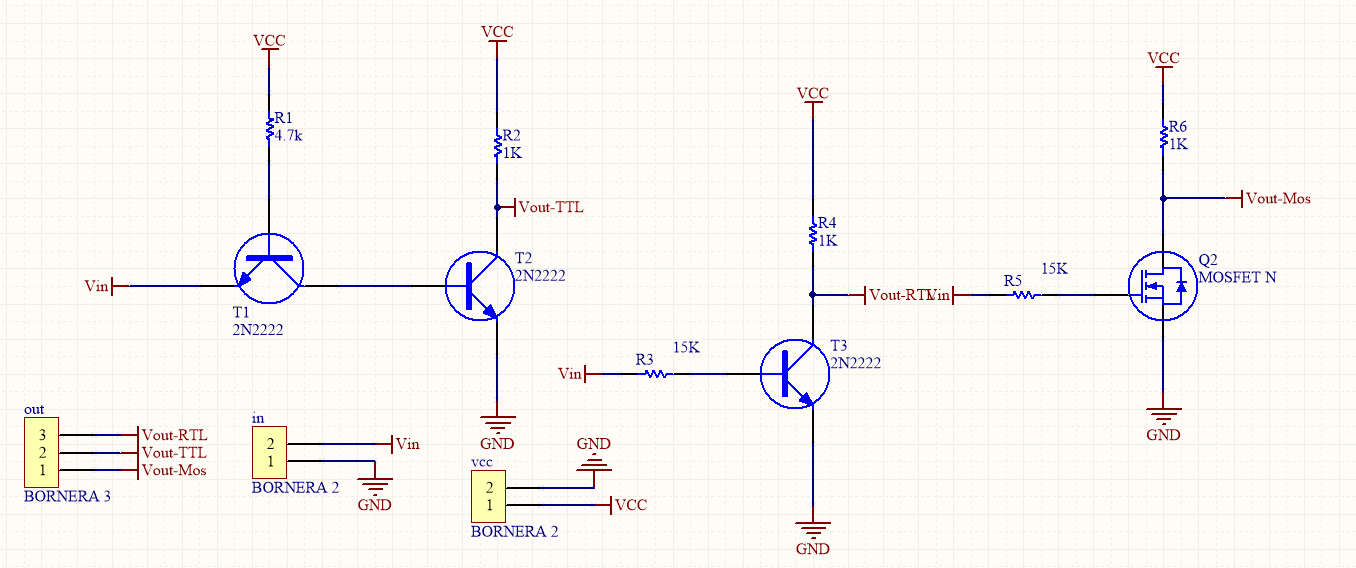
\includegraphics[width=0.5\textwidth]{ImagenesEjercicio1/Esquematico.PNG} \ \ \ \
	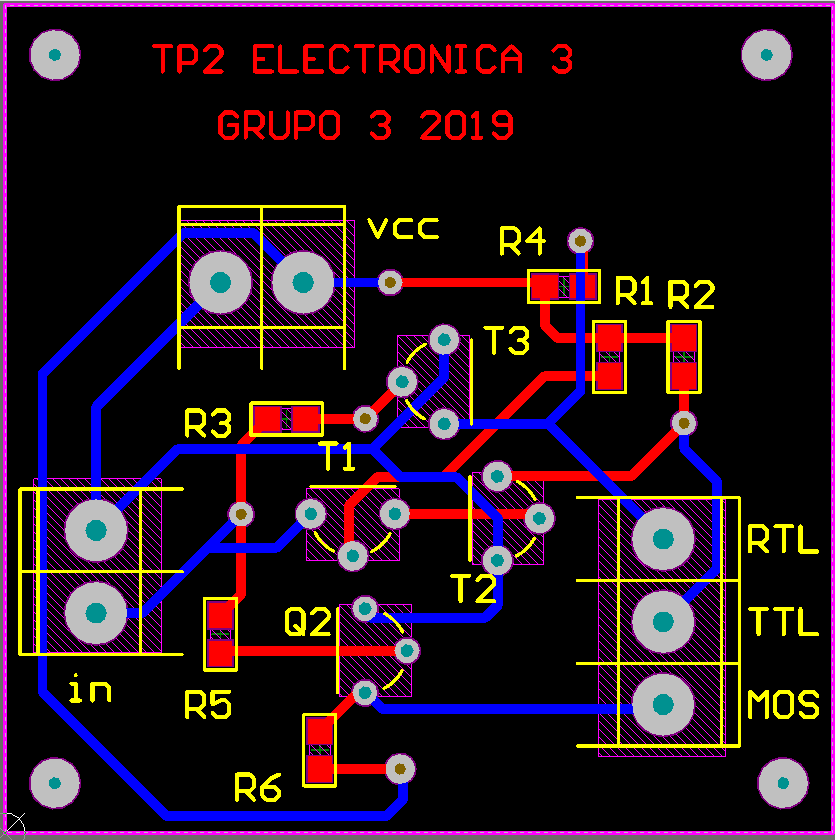
\includegraphics[width=0.3\textwidth]{ImagenesEjercicio1/PCB.PNG}
	\caption{Esquemático y PCB realizados en Altium.}
	\label{fig:esquematico}
\end{figure}

\subsection{Observables de interés.}
\label{sec:Obs}

Se seleccionaron como observables de interés los siguientes parámetros:
\begin{enumerate}
\item \label{VIH} High-level input voltage. 
\item \label{VIL} Low-level input voltage.
\item \label{VOH} High-level output voltage.
\item \label{VOL} Low-level output voltage.
\item \label{NM} Noise Margin.
\item \label{PHL} Propagation delay High to Low.
\item \label{PLH} Propagation delay Low to High.
\item \label{THL} Transition delay High to Low.
\item \label{TLH} Transition delay Low to High.
\item \label{MOC} Maximum output current.
\end{enumerate}

Las mediciones de estos observables se realizaron de la siguiente manera. Para las mediciones de (\ref{VIH}), (\ref{VIL}), (\ref{VOH}), (\ref{VOL}) y (\ref{NM}) se utilizó una rampa, la cual varía desde un valor ligeramente inferior a $0 \ V$ hasta $5 \ V$. Esto se debe a que, dado que se utilizó una rampa periódica, existe un salto al finalizar cada período, el cual representa altas frecuencias que causan problemas. Es decir, considerando el pequeño intervalo de tiempo en el cual la tensión es menor a $0 \ V$, se observó una serie de oscilaciones hasta alcanza a estabilizar la señal. La figura (\ref{fig:medramp}) es un ejemplo de una de las mediciones.
\begin{figure}[H]	
	\centering
	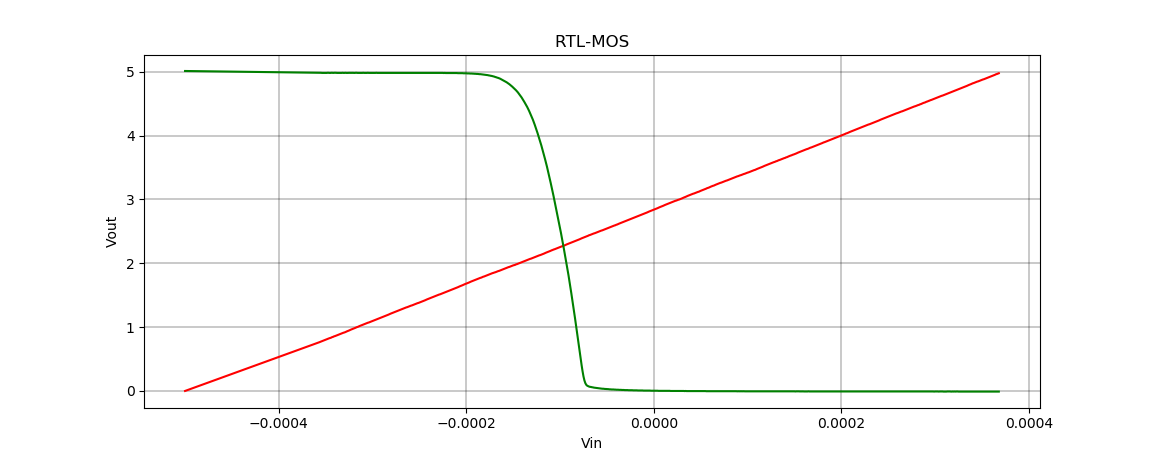
\includegraphics[width=0.9\textwidth]{ImagenesEjercicio1/DC-SWEEP/MedicionRampa.PNG}
	\caption{Medición niveles de tensión.}
	\label{fig:medramp}
\end{figure}

A partir de esta medición, se tomó el módulo de las señales y se graficó la señal de entrada en función de la salida, como se ve a continuación.
\begin{figure}[H]	
	\centering
	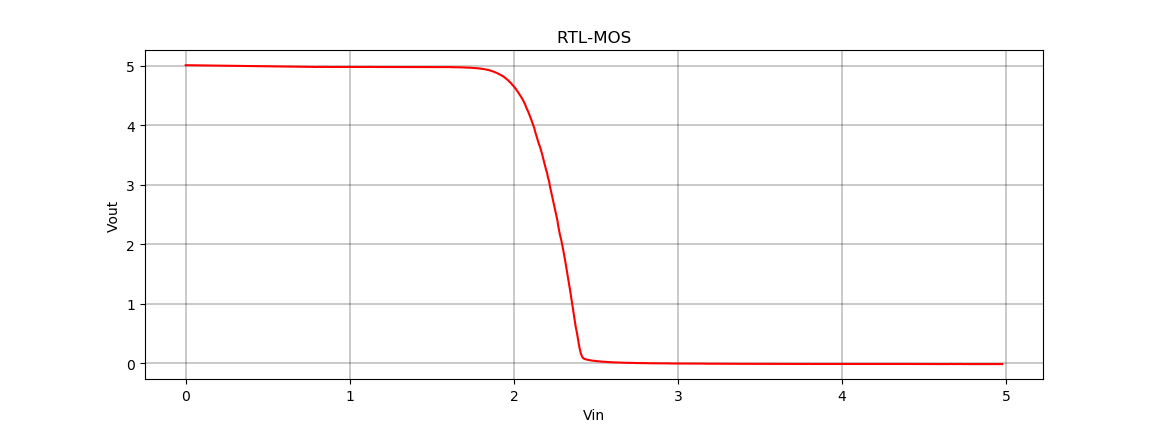
\includegraphics[width=0.9\textwidth]{ImagenesEjercicio1/DC-SWEEP/EntradaSalida.PNG}
	\caption{Medición entrada-salida.}
	\label{fig:medinout}
\end{figure}

Luego, a partir de esta imagen, se buscó el punto donde la pendiente es 45$^{\circ}$. Es así se obtuvo (\ref{VIH}), (\ref{VOH}), (\ref{VIL}) y (\ref{VOL}). Realizando la resta de (\ref{VIH}) con (\ref{VOH}), y de (\ref{VIL}) con (\ref{VOL}) se obtienen los márgenes de ruido (\ref{NM}).

Luego para (\ref{PHL}), (\ref{PLH}), (\ref{THL}) y (\ref{TLH}) se midió la salida, con una cuadrada a la entrada como se ve en la siguiente figura:
\begin{figure}[H]	
	\centering
	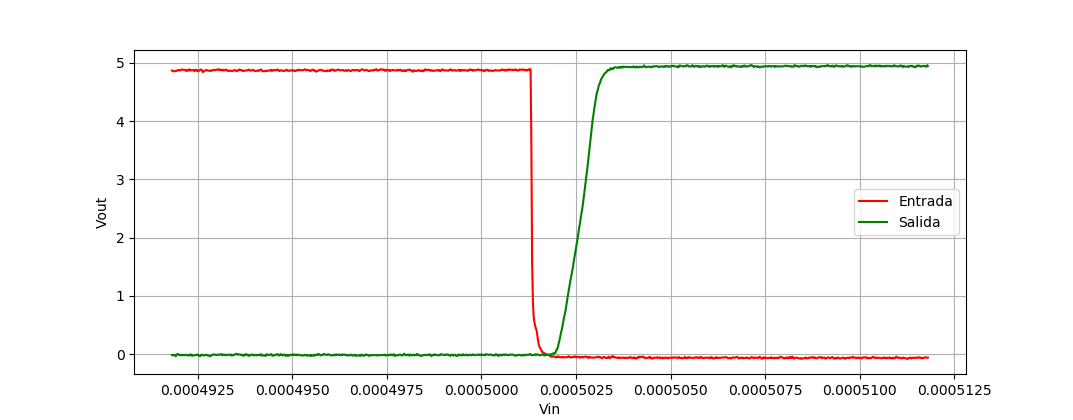
\includegraphics[width=0.9\textwidth]{ImagenesEjercicio1/DC-SWEEP/0t1mtl.PNG}
	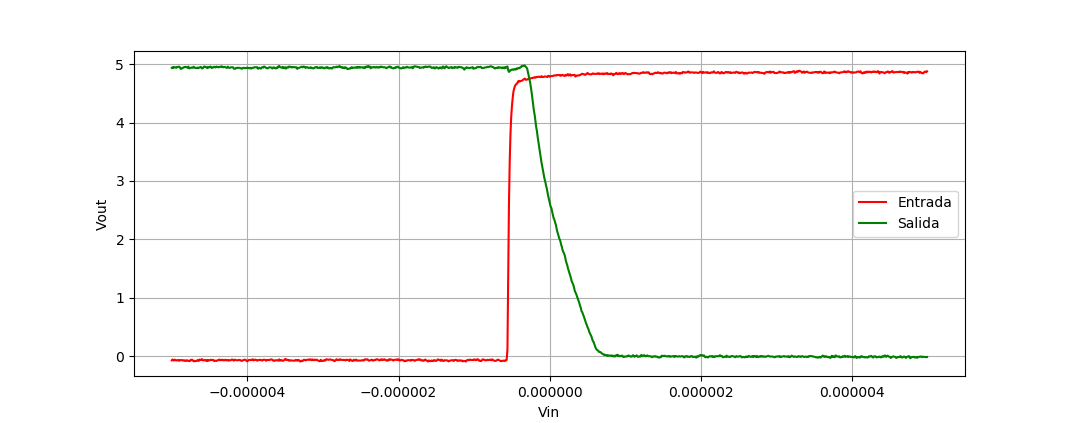
\includegraphics[width=0.9\textwidth]{ImagenesEjercicio1/DC-SWEEP/1t0mtl.PNG}
	\caption{Medición tiempo de propagación y transición.}
	\label{fig:MedicionTiempos}
\end{figure}

Tomando el tiempo de propagación medido al 50\% de la señal y el tiempo de transición medido entre el 10 $\sim$ 90 \%, se buscó obtener el tiempo de propagación existente en una medición. Este resultado dio un valor menor al tiempo de rise del osciloscopio. Dicho valor debe ser interpretado como una cota del tiempo y no el valor exacto. 

Finalmente se colocó un trimmer de $50 \ k\Omega$ utilizándolo como carga, variando su impedancia hasta que el valor de tensión de la salida se encuentre por debajo del High Level Output Voltage. A partir de este valor de tensión y la resistencia del trimmer, se obtiene la corriente máxima de salida.
\begin{figure}[H]	
	\centering
	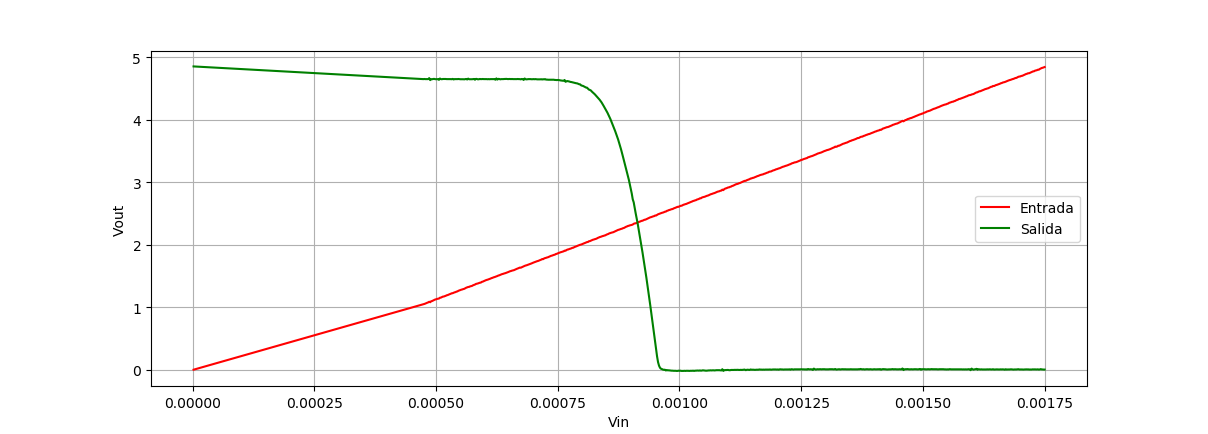
\includegraphics[width=0.9\textwidth]{ImagenesEjercicio1/DC-SWEEP/OutputCurrent.PNG}
	\caption{Medición corriente máxima de salida.}
	\label{fig:OutputCurrent}
\end{figure}

\subsection{Análisis de resultados.}
Para realizar una comparación entre los modelos propuestos, se utilizarán los observables de interés definidos en la sección (\ref{sec:Obs}), confeccionando la siguiente tabla:
\begin{table}[H]
\centering
\begin{tabular}{c|ccc}
\hline
\multicolumn{4}{|c|}{\textit{Sin carga}}                                                                          \\ \hline
\multicolumn{1}{|c|}{\textbf{Tecnología}} & \textbf{RTL}   & \textbf{RTL-MOS} & \multicolumn{1}{c|}{\textbf{TTL}} \\ \hline
High-level input voltage                  & 864 mV         & 2.49 V           & 595 mV                            \\
Low-level input voltage                   & 454 mV         & 1.95 V           & 413 mV                            \\
High-level Output voltage                 & 4.96 V         & 4.89 V           & 4.96 V                            \\
Low-level Output voltage                  & 191 mV         & 72.1 mV          & 34.5mV                            \\
Noise Margin High                         & 4.01 V         & 2.34 V           & 4.37 V                            \\
Noise Margin Low                          & 263 mV         & 1.88 V           & 378 mV                            \\
Propagation delay High to Low             & 76.93 nS       & 569.51 nS        & 1.82 nS                           \\
Propagation delay Low to High             & 2.0489 $\mu S$ & 1.33 $\mu S$     & 535 nS                            \\
Transition delay High to Low              & 87.28 nS       & 734.4 nS         & 38.36 nS                          \\
Transition delay Low to High              & 605 nS         & 909 nS           & 307 nS                            \\
Maximum output current                    & 184.4  $\mu A$ &    217 $\mu A$              &                                  135.5$\mu A$ 	
\end{tabular}
\end{table}
%%%%%%%%%%%%%%%%%%%%%%%%%%%%%%
\begin{table}[H]
\centering
\begin{tabular}{c|ccc}
\hline
\multicolumn{4}{|c|}{\textit{Con carga}}                                                                         \\ \hline
\multicolumn{1}{|c|}{\textbf{Tecnología}} & \textbf{RTL}  & \textbf{RTL-MOS} & \multicolumn{1}{c|}{\textbf{TTL}} \\ \hline
High-level input voltage                  & 840 mV        & 2.48 V           & 627.5 mV                          \\
Low-level input voltage                   & 478.7 mV      & 2.01 V         &    490 mV                         \\
High-level Output voltage                 & 4.98 V        & 4.86 V          & 4.95 V                            \\
Low-level Output voltage                  & 278 mV        & 151 mV           & 72 mV                             \\
Noise Margin High                         & 4.14 V        & 2.52 V           & 4.32 V                            \\
Noise Margin Low                          & 200.7 mV      & 514.9 mV         & 417.3 mV                          \\
Propagation delay High to Low             & 260.7 nS      & 625.7 nS         & 33.6 nS                           \\
Propagation delay Low to High             & 2.615 $\mu S$ & 1.652 $\mu S$    & 1.216 $\mu S$                     \\
Transition delay High to Low              & 183.817 nS    & 417.19 nS        & 73.12 nS                          \\
Transition delay Low to High              & 2.691 $\mu S$ & 2.831 $\mu S$    & 2.687 $\mu S$                     \\
Maximum output current                    &  187.2 $\mu A$             &     216 $\mu A$             &   135.2 $\mu A$                               
\end{tabular}
\end{table}
 

Las diferencias entre los parámetros para las tres tecnologías son notables,
{\begin{center}\color{red} \begin{huge}
PONER CONCLUSIONES \end{huge} \rule{\linewidth}{0.5mm}\end{center} }